\documentclass[
,hyperref={pdfpagelabels=false}
]{beamer}
% Die Hyperref Option hyperref={pdfpagelabels=false} verhindert die Warnung:
% Package hyperref Warning: Option `pdfpagelabels' is turned off
% (hyperref)                because \thepage is undefined.
% Hyperref stopped early

\usepackage{agstyle}
\usepackage{currycode}
\usepackage{tikz}

\newcommand{\ergo}{$\Rightarrow$}
\newcommand{\todo}[1]{\fbox{\sc To do: #1}}

%%%%%%%%%%%%%%%%%%%%%%%%%%%%%%%%%%%%%%%%%%%%%%%%%%%%%%%%%%%%%%%%%%%%%%%%%%%%%%%%

\title[Search Strategies for FLP]
{Search Strategies for Functional Logic Programming}

\date[ATPS 2012]{ATPS 2012, February 27}

\author[Hanus, Peemöller, \underline{Reck}]{%
\texorpdfstring
  {Michael Hanus \and Björn Peemöller \and \underline{Fabian Reck}}
  {Michael Hanus \and Björn Peemöller \and Fabian Reck}
}

\institute{Kiel University}

\begin{document}

\begin{frame}%---------------
\titlepage
\end{frame}

%%%%%%%%%%%%%%%%%%%%%%%%%%%%%%%%%%%%%%%%%%%%%%%%%%%%%%%%%%%%%%%%%%%%%%%%%%%%%%$$

\section{Introduction}

\begin{frame}[fragile]%-------------------------------------------------------
\frametitle{Functional Logic Programming}
\begin{itemize}
\item Was ist FLP?
\item Nichtdeterminismus => Suchen => Suchstrategien
\item Curry-Folie
\item KiCS2-Überblick
\end{itemize}

\begin{itemize}
\item KiCS2 is a compiler from Curry to Haskell
\item Non-determinism is explicitly represented in
      the data structures
\end{itemize}
\end{frame}

\begin{frame}[fragile]%-------------------------------------------------------
\frametitle{Curry}
\begin{itemize}
\item Überlappende Regeln, Fragezeichen
\item Freie Variablen
\item Constraints
\end{itemize}
\end{frame}

\begin{frame}[fragile]%-------------------------------------------------------
\frametitle{Curry-Implementierungen und Top-Level-Suchen}
\begin{itemize}
\item PAKCS: DFS               ; Prolog
\item MCC  : DFS               ; C
\item KiCS : DFS, BFS          ; Unsafe Haskell
\item KiCS2: DFS, BFS, IDS, PAR; Haskell, easily extensible
\end{itemize}
\end{frame}

\section{Search Strategies}

\begin{frame}[fragile]%-------------------------------------------------------
\frametitle{Darstellung des Suchraums als Datenstruktur in KiCS2}
\begin{itemize}
\item Hinweis auf Laziness
\item Grafik
  \begin{itemize}
  \item Curry-Ausdruck
  \item Korrespondierer Suchraum
  \item Evtl. noch Datenstruktur
  \end{itemize}
\end{itemize}
\end{frame}

\begin{frame}[fragile]%-------------------------------------------------------
\frametitle{Berechnung des Suchraums}
\begin{itemize}
\item Normalformberechnung
\item Call-time-choice durch IDs
\end{itemize}
\end{frame}

\begin{frame}[fragile]%-------------------------------------------------------
\frametitle{Suchstrategien}

\begin{itemize}
  \item Based on tree representation of search space
  \item Strategies only extract values
  \item Available: depth-first, breadth-first, iterative deepening
\end{itemize}

\begin{haskell}[SearchTree]
data SearchTree a = None
                  | One a
                  | Choice (SearchTree a) (SearchTree a)
\end{haskell}

\begin{haskell}[Depth-first-search using SearchTree]
allValuesDFS :: SearchTree a -> [a]
allValuesDFS None         = []
allValuesDFS (One      x) = [x]
allValuesDFS (Choice x y) = allValuesDFS x ++ allValuesDFS y
\end{haskell}

\end{frame}

\begin{frame}[fragile]%-------------------------------------------------------
\frametitle{Nutzung}
\begin{itemize}
\item printResults als Beispiel für Top-Level-Suche
\item Als eingekapselte Suche, SearchTree als Curry-Struktur
\end{itemize}
\end{frame}

\section{Benchmarks}

\begin{frame}%----------------------------------------------------------------
\frametitle{Benchmark: Non-Deterministic Permutation Sort}
Program: permutation sort of a list with 15 values
\begin{center}
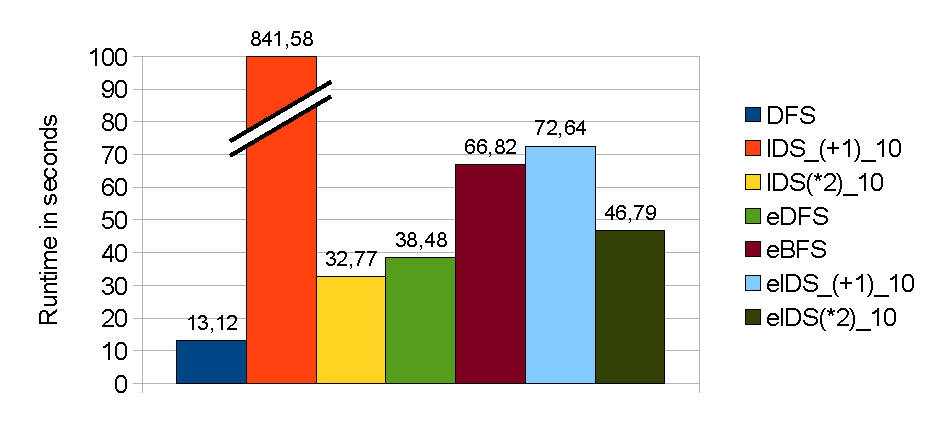
\includegraphics[width=11cm]{gfx/permsort}
\end{center}
\begin{itemize}
\item DFS/eDFS: Overhead durch Suchbaum, Faktor 3
\item $\text{IDS}_{10}^{+1}$ is very slow due to the linear search space
\item $\text{eIDS}_{10}^{+1}$ profits from sharing the search tree
\item IDS(+1)/IDS(*2): Overhead durch Gewährleistung von CTC
\item IDS(*2)/eIDS(*2): Overhead durch Suchbaum, Faktor 1,5
\item IDS(+1)/eIDS(+1). \todo{Aussage}
\end{itemize}
\end{frame}

\begin{frame}[fragile]%-------------------------------------------------------
\frametitle{Benchmark: Last}
Program: halve the Peano number $1600$ by inverting addition
\begin{center}
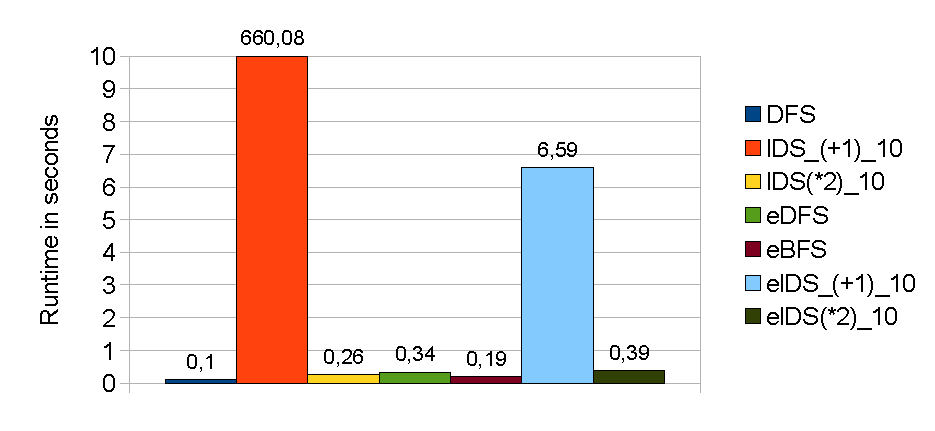
\includegraphics[width=11cm]{gfx/last}
\end{center}

\todo{Laufzeit von BFS erklären}
\end{frame}

\begin{frame}[fragile]%-------------------------------------------------------
\frametitle{Benchmark: NDNums}
\todo{IDS ist voll gut!}
\end{frame}

\section{Conclusion}

\begin{frame}[fragile]%-------------------------------------------------------
\frametitle{Conclusion}

\begin{itemize}
\item Vermeidung von (Problemen bei Festlegung auf DFS)
\item Vorstellung unseres Ansatzes
\item Erste praktische Ergebnisse
\item Vollständige Suchstrategien sind eine ernstzunehmende Alternative zu DFS
\end{itemize}

\end{frame}

\begin{frame}[fragile]%-------------------------------------------------------
\frametitle{Future Work}

\begin{itemize}
\item Untersuchung komplexerer Programme (vllt. sogar reale Programme?)
\item Untersuchung des Speicherverhaltens
\item Untersuchung weiterer Suchstrategien
\end{itemize}

\end{frame}

\end{document}
